\changecolours{ScoutNavy}
\section{O Teorema PACELC}

% ------------------------------------------------------------------------------
\twocolframe[title={Por que o Teorema CAP é Insuficiente no Dia a Dia?},leftcol=7cm,rightcol=7cm]{%
  \alert{O Ponto Cego de Eric Brewer}\par
  \itemseps[topsepi=2mm,itemsepi=3mm,labelsep=2mm,leftmargini=4mm]
  \begin{itemize}
    \item Em 2012, o pesquisador \textbf{Daniel J. Abadi} (Yale University) publicou um artigo seminal na IEEE:
    \item \textit{``Consistency Tradeoffs in Modern Distributed Database System Design: CAP is Only Part of the Story''}.
    \item \textbf{A Pergunta Crítica:} O que acontece quando \textbf{NÃO} há partição de rede?
  \end{itemize}
}{%
  \alert{A Realidade da Nuvem Moderna}\par
  \itemseps[topsepi=2mm,itemsepi=3mm,labelsep=2mm,leftmargini=4mm]
  \begin{itemize}
    \item Em provedores de ponta (AWS, Google Cloud, Azure), o cluster opera em estado normal durante \textbf{99,99\% do tempo}!
    \item O CAP é completamente mudo sobre o comportamento do sistema durante 99,99\% da sua vida útil.
    \item Mesmo sem falha de rede, existe um dilema feroz entre \textbf{Velocidade (Latência)} e \textbf{Coerência (Consistência)}.
  \end{itemize}
}

% ------------------------------------------------------------------------------
\twocolframe[title={A Formulação Mnemônica do Teorema PACELC},leftcol=7cm,rightcol=7cm]{%
  \alert{A Equação Arquitetural de Abadi}\par
  \vspace{0.2cm}
  {\small \textbf{Se houver Partição de Rede (\alert{P}):}}
  \begin{itemize}
    \item Escolha entre Disponibilidade (\textbf{\color{ScoutGreen}A}) ou Consistência (\textbf{\color{ScoutNavy}C}).
  \end{itemize}
  \vspace{0.2cm}
  {\small \textbf{Senão (\alert{Else - E}) em Operação Normal:}}
  \begin{itemize}
    \item Escolha entre Baixa Latência (\textbf{\color{ScoutBlue}L}) ou Consistência (\textbf{\color{ScoutNavy}C}).
  \end{itemize}
}{%
  \alert{As 4 Combinações Possíveis}\par
  \itemseps[topsepi=1.5mm,itemsepi=2.5mm,labelsep=2mm,leftmargini=4mm]
  \begin{itemize}
    \item \textbf{PA/EL:} Prioriza alta disponibilidade na partição e latência ultrabaixa no dia a dia (\textit{Cassandra, DynamoDB}).
    \item \textbf{PC/EC:} Prioriza consistência sempre, pagando o custo de esperar confirmações síncronas (\textit{MongoDB com maioria, RDBMS}).
    \item \textbf{PC/EL:} Consistente na partição, mas otimizado para baixa latência local no dia a dia (\textit{Redis, MongoDB w=1}).
  \end{itemize}
}

% ------------------------------------------------------------------------------
\begin{frame}{A Árvore Decisória Completa do Teorema PACELC}
  \vspace{-0.3cm}
  \makebox[\linewidth][c]{%
    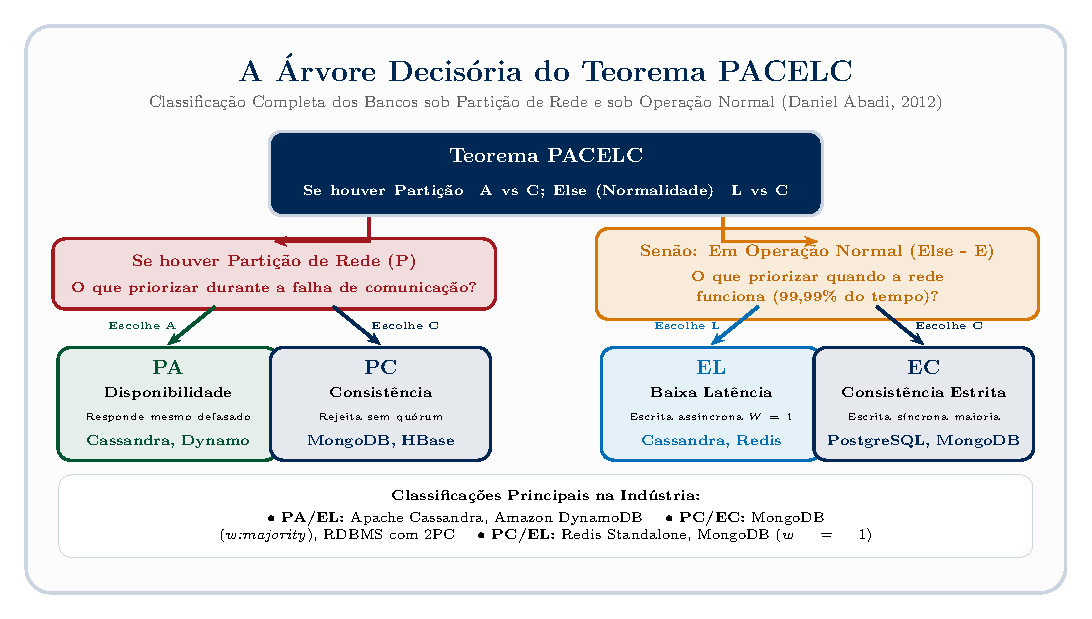
\includegraphics[width=14.0cm,height=4.8cm,keepaspectratio]{figuras/fig_pacelc_arvore.pdf}%
  }\par
  \vspace{0.15cm}
  \centering
  {\footnotesize \textbf{Visão Prática:} \textcolor{ScoutNavy}{O Teorema PACELC mapeia o comportamento do banco tanto na crise (P) quanto no estado normal (Else).}}
\end{frame}

% ------------------------------------------------------------------------------
\twocolframe[title={Exemplo Analítico: O Custo Físico da Consistência},leftcol=7cm,rightcol=7cm]{%
  \alert{Cenário de Negócio Pareado}\par
  \itemseps[topsepi=1.5mm,itemsepi=2.5mm,labelsep=2mm,leftmargini=4mm]
  \begin{itemize}
    \item Cluster com 3 nós em data centers distintos:
    \item Nó 1 (Local): $RTT_1 = 1{,}5 \text{ ms}$ (rack local).
    \item Nó 2 (Fortaleza): $RTT_2 = 45{,}0 \text{ ms}$ (regional).
    \item Nó 3 (Tauá): $RTT_3 = 58{,}0 \text{ ms}$ (interior).
    \item $RTT$ (\textit{Round-Trip Time}): tempo de ida e volta.
  \end{itemize}
}{%
  \alert{Cálculo Analítico de Latência}\par
  \itemseps[topsepi=1.5mm,itemsepi=2.5mm,labelsep=2mm,leftmargini=4mm]
  \begin{itemize}
    \item \textbf{Estratégia PA/EL (Escrita Local $W=1$):}
      $$T_{\text{EL}} = RTT_1 + 0{,}3 = \mathbf{1{,}8\text{ ms}}$$
    \item \textbf{Estratégia PC/EC (Escrita Síncrona Maioria):}
      $$T_{\text{EC}} = \max_i(RTT_i) + 2{,}0 = \mathbf{60{,}0\text{ ms}}$$
    \item \textbf{Trade-off Físico:} A consistência estrita custa $\approx \mathbf{33{,}3\times}$ mais tempo de resposta!
  \end{itemize}
}

% ------------------------------------------------------------------------------
\begin{frame}[fragile]{Demonstração Pareada em Python: Simulação PACELC}
\vspace{-0.3cm}
\begin{lstlisting}
# RTT = Round-Trip Time em milissegundos
rtt_local = 1.5; rtt_fortaleza = 45.0; rtt_taua = 58.0

# PA/EL: Confirmacao imediata no primario local (W=1)
tempo_el = rtt_local + 0.3

# PC/EC: Confirmacao sincrona aguardando quorum
tempo_ec = max(rtt_local, rtt_fortaleza, rtt_taua) + 2.0

print(f"Latencia PC/EC (Consistencia Estrita) : {tempo_ec:.1f} ms")
print(f"Latencia PA/EL (Baixa Latencia W=1)   : {tempo_el:.1f} ms")
print(f"Aceleracao no modelo EL               : {tempo_ec/tempo_el:.1f}x mais rapido!")
\end{lstlisting}
\vspace{-0.1cm}
\centering
{\scriptsize \textcolor{ScoutNavy}{\textbf{Tomada de Decisão:}} Para IoT/curtidas, escolha \textbf{EL}. Para financeiro, use \textbf{EC}.}
\end{frame}
